\documentclass[../main.tex]{subfiles}
 
\begin{document}

% in one paragraph, provide an overview of the methodology including a complete formal definition of the ML task and the relationship between an input and the output (possibly using a math description), describe the data, explain how performance will be analyzed

This research shows that \ac{can} data uniquely identifies a vehicle. We train two different deep learning models---one a standard \ac{mlp} and the other a \ac{cnn}---to determine how well a model can distinguish between \ac{can} data samples from different vehicles. Every sample in the dataset, which comes from \ac{ornl} and from \cite{Stone2018}, contains 1) 1,024 sequential bytes of \ac{can} data and 2) a vehicle ID. Input to the models consist of the data bytes; the model then predicts the vehicle ID and compares its output to the true vehicle IDs. This is thus a supervised classification problem, and so it is likely that supervised techniques can learn to discriminate between samples from distinct vehicles.

% overview of the methodology

The remainder of this section discusses the data in detail: its nature and origins, the cleanup and formatting process, and the classes and their distributions. Additionally, this section describes the deep learning models employed, including the architectures and the model-fitting and evaluation processes. 

\subsection{Data}\label{methodology:data}

% describe where the data came from

This research uses data from two sources. \acl{ornl} recently conducted at least 52 \ac{can} data captures on nine different vehicles. Some of those 52 captures contain sensitive information, so the lab shared the data from the 34 non-confidential captures. Additionally, \cite{Stone2018} conducted one capture on each of 11 different vehicles. In total, this research uses 2.44 gigabytes of data from \ac{ornl} and another 230 megabytes of Stone's \ac{can} data. Table \ref{tab:vehicles} displays metadata for the 20 vehicles in the dataset.

\begin{table}
    \caption{Make, Model, and Year for the Twenty Vehicles}
    \centering
    \label{tab:vehicles}
    \begin{tabular}{|c|c|c|c|}
    \hline
    \textbf{Vehicle} & \textbf{Make} & \textbf{Model} & \textbf{Year} \\
    \hline
    1   & Toyota    & Tacoma    & 2008 \\
    2   & Toyota    & Corolla   & 2009 \\
    3   & Nissan    & Leaf      & 2011 \\
    4   & Ford      & C-Max     & 2013 \\
    5   & Chevrolet & Volt      & 2015 \\
    6   & Ford      & F-150     & 2014 \\
    7   & Ford      & Fusion    & 2016 \\
    8   & Subaru    & WRX       & 2017 \\
    9   & Subaru    & Outback   & 2009 \\
    101 & Chevrolet & Cobalt    & 2009 \\
    102 & Chevrolet & Silverado & 2011 \\
    103 & Dodge     & 1500      & 2014 \\
    104 & Ford      & F-150     & 2017 \\
    105 & Ford      & Focus     & 2010 \\
    106 & Honda     & Accord    & 2012 \\
    107 & Honda     & Accord    & 2015 \\
    108 & Nissan    & 370Z      & 2015 \\
    109 & Nissan    & XTERRA    & 2010 \\
    110 & Saab      & 9-7X      & 2009 \\
    111 & Toyota    & Corolla   & 2009 \\
    \hline
    \end{tabular}
\end{table}

% describe data cleanup

A large \ac{csv} file stores the data. Each of the 44,893,238 rows in this file represents one \ac{can} message, and each row contains:

\begin{itemize}
    \item a \texttt{capture\_id} and a \texttt{vehicle\_id}, which identify the message's origin,
    \item a \texttt{timestamp} relative to the start of the capture,
    \item an \texttt{arbitration\_id}, which serves as the vehicle's identifier of the message's contents,
    \item a \texttt{dlc}, or \textit{data length code}, which indicates how many bytes of data the message contains,
    \item the hexadecimal \texttt{data} itself,
    \item and the vehicle's \texttt{make}, \texttt{model}, and \texttt{year}.
\end{itemize}

The messages in this \ac{csv} file are not immediately suitable for deep learning. Each message contains no more than eight data bytes (and many contain fewer), and it is extremely unlikely that so little information can uniquely identify a vehicle. Additionally, disparate arbitration IDs typically contain disparate information. For example, arbitration ID 704 might detail a vehicle's instantaneous velocity while 1A3 contains the same vehicle's gear setting. A model that does not discriminate between the various IDs---that is, a model that trains on the messages as they appear in the \ac{csv} file---is not likely to learn the nuances of a given vehicle's \ac{can} traffic.

To address this issue, we build a set of data samples, where each sample contains 1,024 bytes of sequential \ac{can} data from one arbitration ID of one capture. Specifically, for each arbitration ID in each capture, we sort the messages by timestamp before splitting all hex data into a list of hex bytes, converting the hex bytes into integers, and dividing the list into samples of 1,024 integers. Because each integer represents one byte of \ac{can} data, each sample contains $8*1024=8192$ data bits. Then, for arbitration IDs with at least one full sample\footnotemark[2], we write each sample and the associated vehicle ID to a new \ac{csv} file. This makes it more likely that a) each sample contains sufficient information and that b) the underlying \ac{can} data structure is preserved.

\footnotetext[2]{Arbitration IDs without at least one full sample are not likely to positively contribute to the model, so these IDs are ignored.}

% how many observations?
% how many classes? what is the distribution of observations?

This new \ac{csv} file contains 297,244 samples from 1,012 arbitration IDs of 20 vehicles. Table \ref{tab:sample-metadata} illustrates the distributions of arbitration IDs and samples over all vehicles (the number of arbitration IDs for a given vehicle is innate; the number of samples, on the other hand, depends primarily on the length of the data capture). Clearly, Vehicles 3, 5, and 7 contain a large majority of all samples, and Vehicle 3 contains nearly half. As described in Section \ref{sec:model-fitting}, we address this class imbalance during model training.

\begin{table}
    \caption{Number of Arbitration IDs and samples Per Vehicle}
    \centering
    \label{tab:sample-metadata}
    \begin{tabular}{|c|r|r|r|r|}
    \hline
    \textbf{Vehicle} & \textbf{ArbIDs} & \textbf{samples} & \textbf{Proportion} \\
    \hline
    1   & 8   & 4440   & 1.49  \% \\
    2   & 47  & 6895   & 2.32  \% \\
    3   & 49  & 141841 & 47.72 \% \\
    4   & 103 & 14631  & 4.92  \% \\
    5   & 112 & 43377  & 14.59 \% \\
    6   & 79  & 9511   & 3.20  \% \\
    7   & 124 & 35142  & 11.82 \% \\
    8   & 35  & 5018   & 1.69  \% \\
    9   & 21  & 8211   & 2.76  \% \\
    101 & 29 & 4102    & 1.38  \% \\
    102 & 50 & 1824    & 0.61  \% \\
    103 & 62 & 1756    & 0.59  \% \\
    104 & 78 & 2182    & 0.73  \% \\
    105 & 24 & 3791    & 1.28  \% \\
    106 & 28 & 1695    & 0.57  \% \\
    107 & 42 & 2198    & 0.74  \% \\
    108 & 38 & 3020    & 1.02  \% \\
    109 & 26 & 2553    & 0.86  \% \\
    110 & 19 & 2974    & 1.00  \% \\
    111 & 38 & 2083    & 0.70  \% \\
    \hline
    \end{tabular}
\end{table}

% what info is contained in the supervised learning label?

Table \ref{tab:samples} presents a few example data samples. The deep learning model receives these samples as input and attempts to predict the vehicle that generated each sample; the model does \textit{not} receive the capture or arbitration ID. This ensures the model cannot simply learn which captures/arbitration IDs map to each vehicle.

\begin{table}
    \caption{Examples of \ac{can} Data samples}
    \centering
    \label{tab:samples}
    \begin{tabular}{|c|c|c|c|}
    \hline
    \textbf{Vehicle} & \textbf{Capture} & \textbf{ArbID} & \textbf{Data} \\
    \hline
    3   & 8   & 1532 & 074 166 111 254 255 240 254 \ldots \\
    7   & 24  & 535  & 003 212 003 209 003 199 003 \ldots \\
    108 & 108 & 292  & 255 248 000 128 015 254 030 \ldots \\
    111 & 111 & 624  & 026 000 065 073 073 064 000 \ldots \\
    \hline
    \end{tabular}
\end{table}

\subsection{Model Architecture}

% describe the deep learning task

To demonstrate that a given vehicle's \ac{can} data uniquely identifies said vehicle, we train and compare deep learning models on multiple data samples. As described in Section \ref{methodology:data}, each sample contains sequential \ac{can} data from one arbitration ID of one data capture, and each is labeled with one of 20 vehicles, so this is a supervised classification problem.

% what are the high-level characteristics of the task and input data that inform the selection of the architecture?

Using a \acl{mlp} to classify vehicles is a bit of a naive approach, but we wish to present the naive approach's performance to demonstrate that an attacker does not need overly complex methods to adequately classify vehicles. Each \ac{can} sample contains 1,024 data bytes, so the \ac{mlp} receives $1024 * 8 = 8192$ bits as input and outputs one of the 20 classes. Section \ref{model:mlp} describes the \ac{mlp} in detail.

We also present a more complex approach---a \acl{cnn}---to demonstrate that a sophisticated attacker can achieve increased performance over the naive approach. Because each sample contains sequential, one-dimensional data, and because the task at hand is classification, the \ac{cnn} utilizes one-dimensional convolutional layers. In testing, the \ac{cnn} receives one sample as input and outputs one of the 20 classes. Section \ref{model:cnn} presents the details of the \ac{cnn}.

\subsubsection{The Multilayer Perceptron}\label{model:mlp}

% what is the overall model type?
% provide a per-layer architecture diagram
% provide a count of the total trainable parameters
% provide a description of how you made model parametrization decisions

We test multiple hyperparameter configurations to identify the best \ac{mlp}; the left panel of Figure \ref{fig:best-archs} displays this model. It has three hidden layers, each of which has 512 nodes and uses a \texttt{relu} activation function. The output layer contains twenty nodes---one for each vehicle in the dataset---and uses a \texttt{softmax} activation function. We compile the model with an Adam optimizer of learning rate $lr = 0.001$ and a categorical cross-entropy loss function. The model has 1,060,372 parameters, all of which are trainable.

\begin{figure}
    \centerline{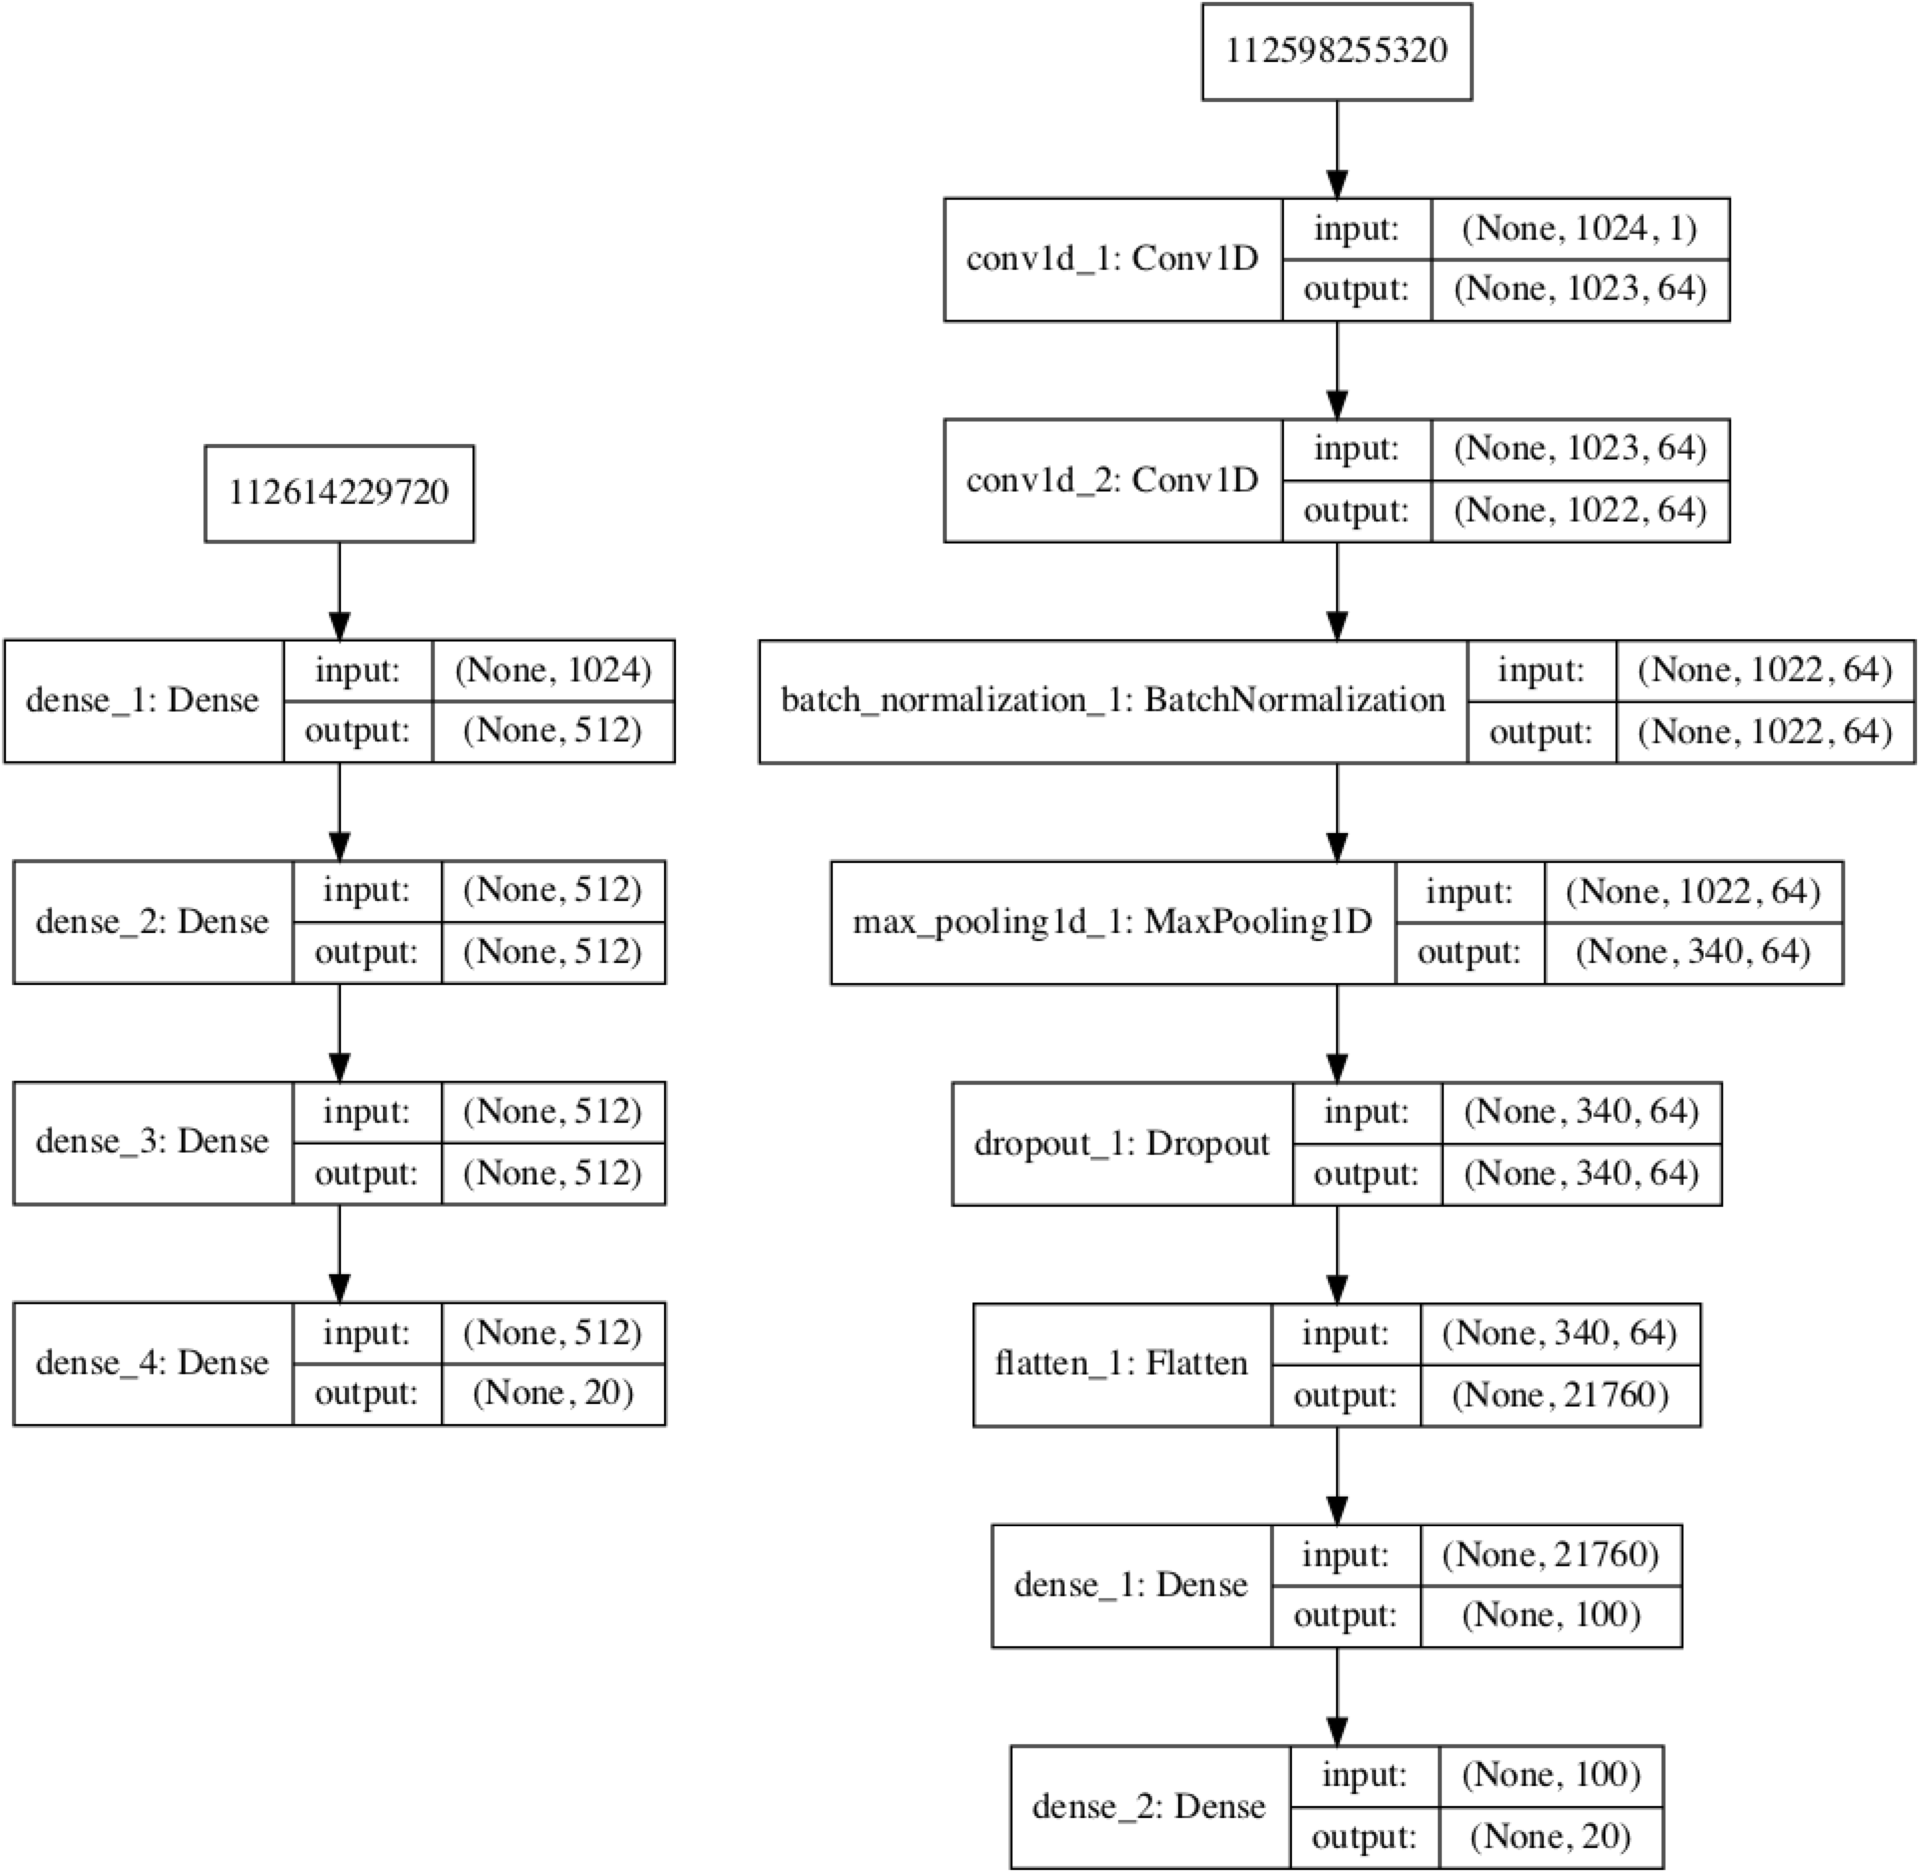
\includegraphics[scale=0.7]{architectures.png}}
    \caption{The best architecture identified in an iterative model evaluation process. \textit{Left:} \acl{mlp}; \textit{Right:} \acl{cnn}.}
    \label{fig:best-archs}
\end{figure}

Every \ac{mlp} implementation utilizes this basic architecture. In total, we test 27 \ac{mlp} architectures; Table \ref{tab:mlp-archs} lists the various options for each hyperparameter used during model construction.

\begin{table}
    \caption{Hyperparameter Options for \ac{mlp} Construction}
    \centering
    \label{tab:mlp-archs}
    \begin{tabular}{|c|c|}
    \hline
    \textbf{Hyperparameter} & \textbf{Options} \\
    \hline
    Number of hidden layers          & 1, 2, 3             \\
    Number of nodes per hidden layer & 128, 256, 512       \\
    Optimizer learning rate          & 0.01, 0.001, 0.0001 \\
    \hline
    \end{tabular}
\end{table}

\subsubsection{The Convolutional Neural Network}\label{model:cnn}

% what is the overall model type?
% provide a per-layer architecture diagram
% provide a count of the total trainable parameters
% provide a description of how you made model parametrization decisions

Like with the \ac{mlp}, we test multiple hyperparameter configurations before selecting the best \ac{cnn}. The best model utilizes a typical \ac{cnn} structure consisting of convolutional, pooling, and dropout layers. The right panel of Figure \ref{fig:best-archs} displays the specific architecture. The convolutional layers each use 64 filters with a kernel size of two, the pooling layer pools over three elements at each step, and the dropout layer sets 50\% of its inputs to zero. The convolutional layers and the first dense layer all use a \texttt{relu} activation function; the final dense layer uses \texttt{softmax}. We again compile the model with an Adam optimizer of learning rate $lr = 0.001$ and a categorical cross-entropy loss function. In total, the model has 2,186,824 parameters, and all but 128 are trainable.

Every \ac{cnn} implementation utilizes this basic architecture. In total, we test 18 \ac{cnn} architectures; Table \ref{tab:cnn-archs} lists the various options for each hyperparameter used during model construction.

\begin{table}
    \caption{Hyperparameter Options for \ac{cnn} Construction}
    \centering
    \label{tab:cnn-archs}
    \begin{tabular}{|c|c|}
    \hline
    \textbf{Hyperparameter} & \textbf{Options} \\
    \hline
    Filters per convolutional layer & 32, 64  \\
    Kernel size per filter          & 2, 3, 4 \\
    Pooling size                    & 2, 3, 4 \\
    \hline
    \end{tabular}
\end{table}

\subsection{Model Fitting}\label{sec:model-fitting}

% how are you handling classification on imbalanced classes?

Table \ref{tab:sample-metadata} shows that the classes in the full dataset are significantly imbalanced. For example, nearly 48\% of all samples come from Vehicle 3; one should expect each vehicle to contain about 5\% of the samples. To address this imbalance, we use scikit-learn's \texttt{class\_weight} module during model training; this tool adjusts weights to account for the frequency of each class, and thus it ensures that both models can use all training data without unnecessarily suffering from class imbalance. Additionally, we create a second, balanced dataset by randomly sampling $n = 1695$ samples from every vehicle.

% describe techniques used to prevent underfitting/overfitting

Another important tool during model training is Keras's \texttt{EarlyStopping} callback, which limits overfitting. This function monitors validation loss during training and terminates the training if said loss does not improve in 10 epochs. The callback then restores the model to its best possible version. This tool also limits model training time.

% how are you partitioning the data into train/validation/test sets?

To properly train and evaluate the models, we split each dataset into three sets: 60\% of the samples are used in training, 20\% in validation, and 20\% in testing. Scikit-learn's \texttt{train\_test\_split} enables this split by randomly sampling from the dataset. We train each model on the training set, terminate training with the early stopping callback (which monitors the validation set's loss), and evaluate the trained model on the testing set.

% iteration to improve results?
% model tuning/selection? if so, what's the plan?

However, these tools do not guarantee optimality, so we also iteratively improve the models through repeated testing and hyperparameter tuning. A search over a set of possible hyperparameter configurations ensures we can identify the best classifier. In total, we evaluate 27 different \acp{mlp} and 18 different \acp{cnn}. Tables \ref{tab:mlp-archs} and \ref{tab:cnn-archs} depict the hyperparameter options for these models.

\subsection{Model Evaluation \& Analysis}

% comparing models? improving on existing models?

We present results for the \acl{mlp} to demonstrate that an intruder with any understanding of deep learning can use this field to better format \ac{can} attacks. We compare the \ac{mlp}'s performance to that of a \ac{cnn} to show that a sophisticated intruder can use more advanced techniques and achieve better results.

% confusion matrices? ROC/AUC? accuracy? precision? class imbalances?

To evaluate model performance, we compute balanced accuracy for both the balanced and the imbalanced dataset. This metric takes into consideration the various class distributions when computing the classification accuracy. Even for the balanced dataset, this is important: because we randomly sample from the dataset to build the training, validation, and testing sets, each of those three sets could be imbalanced. 

% plan for evaluating errors/residuals?

Additionally, we present confusion matrices to allow for an in-depth analysis of where each model fails. For example, Manufacturer X could use the exact same \ac{can} configuration for different models, so even a well-trained model could fail to distinguish between Manufacturer X's vehicles. These analyses may even imply a similar \ac{can} structure across different makes, so the results of these investigations guide further model modifications and tuning.

% transition paragraph

The remainder of this report details the results of the experiment. Specifically, Section \ref{sec:results} presents and discusses the results and implied performance of the two models. Section \ref{sec:conclusion} describes the implications of these results and suggests a few areas for future research.

\end{document}
